\section{Practical Byzantine Fault \\
Tolerance}

Practical Byzantine Fault Tolerance (PBFT) is an algorithm proposed by Miguel Castro and Barbara Liskov in 1999 in order so solve the problem of reaching Byzantine Fault Tolerance in distributed
systems in a way that the performance inpact remains relatively small. The algorithm is a type of state machine replication which offers liveness and safety in a synchronous or
asynchronous system as long as at most $(n-1)/3$ nodes are simultaneously faulty.\cite{url:pbft}

\subsection{The algorithm}

As already mentioned the algorithm is a form of state machine replication which means the state machine is replicated to different nodes in the system with each replica maintaining bot the current
service state and implementing all available service operations. It is assumed that there are $R=3f+1$ replicas where $f$ is the maximum number of faulty nodes. Each replica is assigned a number
in ${0,...,R-1}$. These replicas then move trough a succession of so called \textit{views} which are just different configurations of the replicas. In each view a replica $p=v\ mod\ R$ is selected
which then represents the \textit{primary} in the current view, while the other replicas represent the \textit{backups}. A view is changed if it is believed that the primary is experiencing a
failure.

\begin{figure}[ht]
\centering
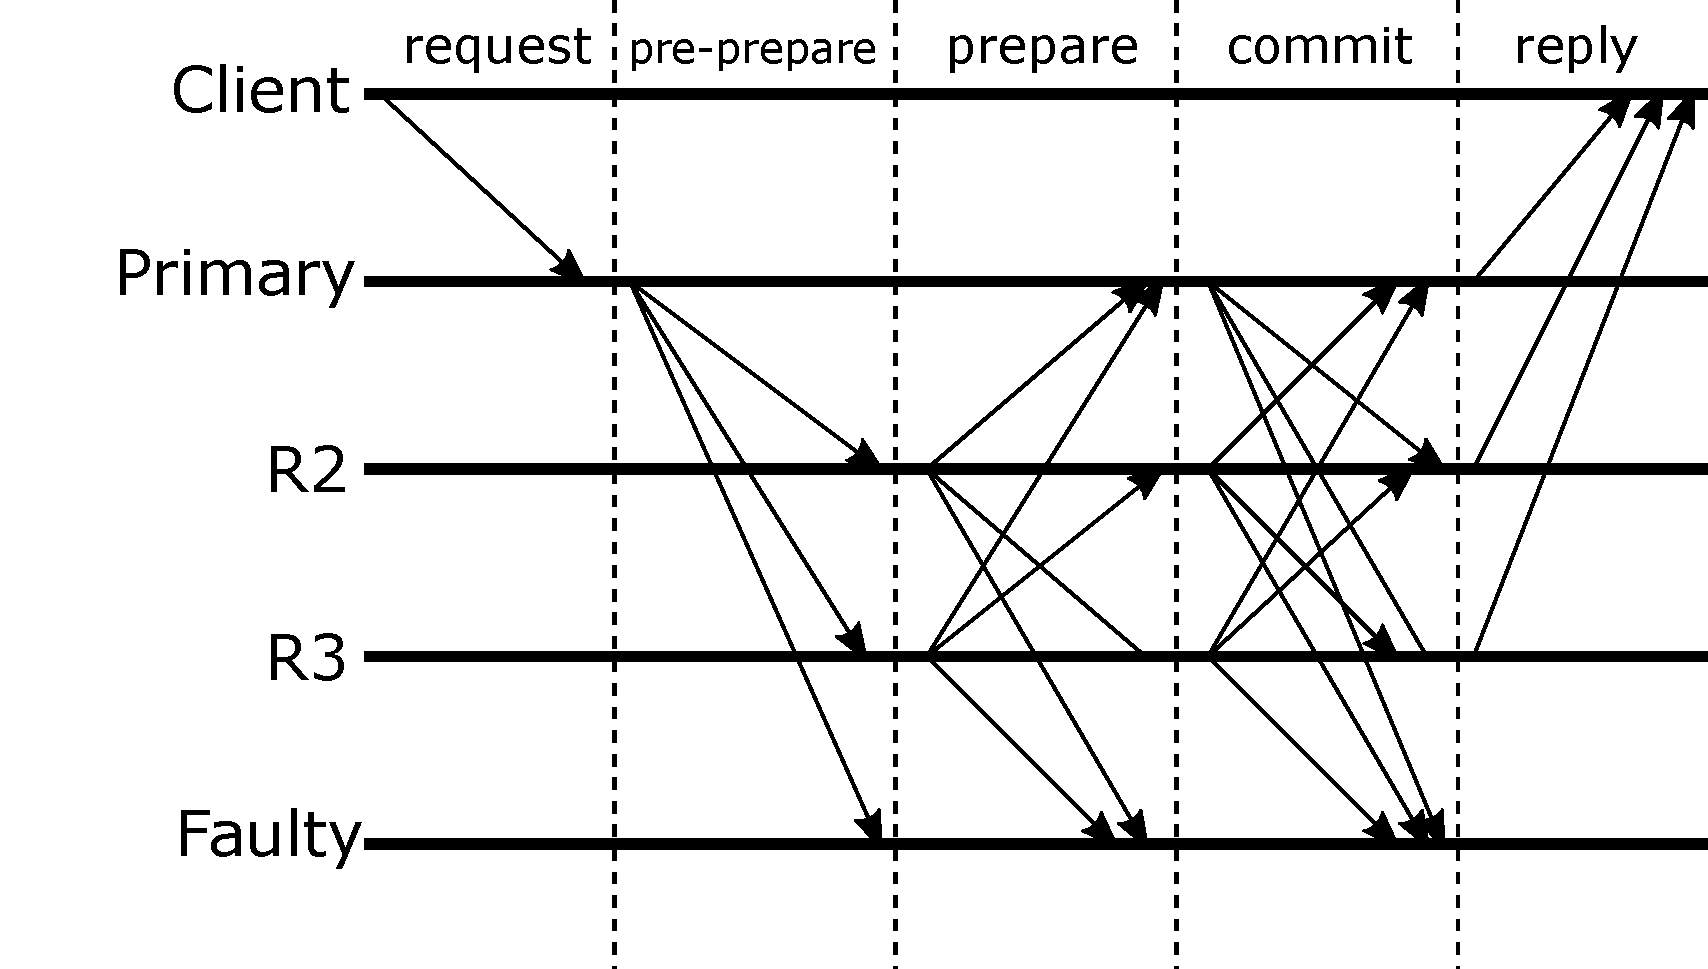
\includegraphics[width=1\columnwidth]{fig/PBFT.pdf}
\caption{Overview of message exchange during PBFT algorithm}
\end{figure}

The algorithm then works roughly as follows: A client sends a request for the execution of a operation by sending a signed request message to the primary. This message contains
the id of the requested operation, a timestamp and the id of the requesting client. As soon as the primary receives the request it starts a three-phase protocol.
In the first, the pre-prepare phase, the primary multicasts a pre-prepare message to all backups. This message contains a sequence number, the current view, the clients request message
and the hash of the clients request message. The whole message is signed by the primary and it is appended to the primary's log.

In the next step each backup checks the pre-prepare message for its validity by checking if the signature and the hash are correct, checking that the message has the same view as the backup and
that it has not accepted a other pre-prepare message with with the same view and sequence number but a different hash. If a backup \textit{i} accepts a pre-prepare message it enters the \textit{prepare}
phase in which it multicasts a prepare message containing the view, the sequence number and the hash from the pre-prepare message as well as the backups id \textit{i}. Both the pre-prepare and
prepare message are also appended to its log. Other replicas receiving such prepare messages accept them and add them to their log as long as the signature, the hash and the view are
valid. A request is then accepted as a \textit{prepared} message, when a replica receives $2f$ prepare messages from other replicas, which match the pre-prepare message and have valid signatures
and hashes. If no more than $f+1$ replicas are faulty this guarantees that the request is valid and should be accepted. As soon as a replica accepts a prepared message, it is again added to its log
and then multicast in a signed commit message again with the view, the sequence number, the hash and the id of the replica. Afterwards the final commit phase is entered.

Receiving replicas add the commit
message to their log as long as the signature and the hash are valid. The request is then considered to be commited-local by a replica if $2f+1$ commits have been received and accepted from
different replicas (including its own). If a request is considered to be commited-local and all requests with a lower sequence number have been executed, the replica will then execute the operation
requested by the client.

\subsection{Application}

The authors of the paper also included the findings of their attempt to implement the algorithm in a real world application. They implemented the algorithm as a replication library and then used this
library to implement a Byzantine-Fault-tolerant NFS file system. They showed that using the algorithm resulted in a only 3\% time increase in operations on the file system, which proves
that the algorithm could be used for real world applications. 
